\documentclass{sig-alternate}
\usepackage{mdwlist}
\usepackage{url}

\begin{document} 

\title{Indoor Navigation and Positioning Using Low Energy Bluetooth}
\subtitle{Dept. of CIS - Senior Design 2013-2014\thanks{Advisor: Boon Thau Loo (boonloo@cis.upenn.edu).}~}
\numberofauthors{2}
\author{
\alignauthor Eric Kim \\ \email{erkim@seas.upenn.edu} \\ Univ. of Pennsylvania \\ Philadelphia, PA
\alignauthor  Aditya Sood\\ \email{asood@seas.upenn.edu} \\ Univ. of Pennsylvania \\ Philadelphia, PA}
\date{10/14/2013}
\maketitle

\begin{abstract}
  \textit{Currently, mobile phones are the primary method of navigation. 
However, indoor positioning and navigation poses a unique problem 
because the GPS satellites normally used to navigate outdoors have
limited use indoors. One solution is using Wifi access points as anchors,
measuring the signal strength and calculating position using trilateration.
Indeed there are companies today that provide the framework for 
such an implementation. However there are certain disadvantages with
using Wifi, namely that there is no context to the position. A location
must be associated with a particular context separately.
    }

  \textit{This project aims to address this issue by implementing a 
different method of indoor positioning, one that uses the recently
released Bluetooth 4.0. With the new APIs released by Google and
Apple in the past few months, we can now use Bluetooth devices
to act as anchors. One key feature of Bluetooth 4.0 is the communication
between devices that is allowed; this will allow us to enrich and 
contextualize position. This peer to peer messaging opens up many
possibilities, ranging from applications in shopping malls to 
emergency response teams.}
\end{abstract}

\section{Introduction}
\label{sec:intro}
 With the widespread availability of the smart phone, individual 
navigation has been refined such that a user can navigate to and 
from a particular address. The standard used today for outdoor 
navigation relies on GPS satellites to track the device location. GPS 
is generally not well suited for indoor use for two reasons - 1. GPS 
does not provide a high level of accuracy, and 2. the GPS signal 
breaks down indoors. So rather than using GPS satellites, indoor 
navigation and positioning has been accomplished largely through 
using networks of nearby "anchors" that have a static, known position. 
Most commonly used anchors today are Wifi networks. The device 
detects a Wifi network with a unique ID; with the wifi access point, 
we can triangulate the exact position of the device. Indeed there are 
several existing companies that will set up the necessary pieces to 
allow for step by step navigation through a shopping mall or a 
departmental store.\footnote{ See meridianapps.com and senionlab.com}

Google and Apple have both introduced a technology called Low 
Energy Bluetooth, also known as BLE or Bluetooth Smart, that 
introduces a new way to navigate indoors. Apple in their recent 
release of iOS7 has included an API called iBeacon, that will use BLE
extensively for the purpose of precise geolocation\cite{apple}. Any "beacon" 
that is set up will be available for general iPhone users to navigate
with; what makes this technology remarkable is that BLE uses very
little energy, as the name suggests, has considerable range, especially
compared to Wifi networks, and most importantly, beacons can be
setup anywhere. Any iPhone device can be set as a beacon, and 
devices designed specifically for the use of becaons can be purchased.
Similarily, Android in their most recent OS release 4.3 has implemented
BLE as well, providing a well defined API\cite{android} to develop upon. 
As of the writing of this paper, only the most recent devices even have 
BLE hardware built in, and on top of that only select devices have the 
OS that provides a native API to utilize BLE, so suffice it to say BLE as a 
method of navigation is still in its early stages.

A method of adding context to position has many important use cases.
One example is in emergency response situations, where location 
awareness is of utmost importance. "Existing indoor navigation solutions
usually rely on pre-installed sensor networks, whereas emergency
agents are interested in fully auto-deployable systems"\cite{renaudin}. 
Indeed the current Wifi implementation requires Wifi access points, a 
data service that computes location, and a location specific context in
order to work correctly. Although this might be feasible for shopping
malls and departmental stores, it does not have much use in a situation
where there is no predefined context. With BLE, all we need to do
is drop a few anchors to detect devices and have the devices transmit
small pieces of data, such as an ID, and we can successfully track
the location.

Existing indoor navigation systems have the problem of high setup
costs and a lack of contextual awareness. Our project will address
this issue by using the aforementioned BLE technology.  "The GATT 
profile is a general specification for sending and receiving short pieces 
of data known as 'attributes' over an LE link. All current Low Energy 
application profiles are based on GATT" \cite{bluetooth}. Using the
GATT profile, contextual awareness is now possible to add anywhere.
Important to note here is that all current Low Energy application 
profiles are based on GATT - this means any device can act as an
anchor, receiving and sending pieces of data, eliminating the lengthy
and costly setup of wifi access points and a framework to manage 
them.

In order to accomplish this implementation, we will need to extensively
test the capabilites of BLE. We need to be familiar with the range and
limitations of the hardware; the range and strength of the bluetooth
signal must be tested. Empirical tests on older versions of Bluetooth
do exist, and we will use this as a benchmark and starting point for our
research and testing\cite{cheung}.


\section{Related Work}
\label{sec:related_work}
Fully functional Indoor navigation apps, although a relatively recent 
invention, have been implemented before. For example, the company
SenionLab provides a way for third parties to integrate an indoor
navigation API to their existing application\cite{senion}\footnote{
SenionLab: The website contains a splendid video demonstrating 
the capabilities of their turn by turn navigation http://senionlab.com}.
The API includes location based advertising, allowing for companies to 
send tailored advertisements to the customers that walk by their store, 
location analytics, the ability to gather data on user behavior and most
importantly, a fully functional step by step navigation system at the
granular level. However, there are some shortcomings that current
indoor navigation apps have in common. Most widespread is the 
dependence on existing Wifi access points as the anchors. Although 
this allows for the application to pinpoint the exact location of the 
device and track it as it moves, it does not provide environmental
awareness. These Wifi based implementations do not carry any 
data about a particular location, such as whether a store carries a 
particular product, or if the store is currently having a sale. A 
fundamental assumption is being made in this case, that is, 
customers already know \textit{where they want to go}, rather than 
\textit{what they want to do}, and this is the fundamental issue
we seek to resolve.

We also cannot forget the costs of implementing a framework that
uses wifi access points. Wifi needs to be set up well in advanced,
and a data service that calculates position must be implemented.
Finally, Wifi has associated costs that the user must invest in, such
as monthly internet charges, maintenance, and an app for users
to download so that they any of the positioning makes sense.

With BLE we no longer have to make this assumption. BLE signal 
transmitters are low cost: for example, for Apple's iBeacon, "beacons"
as they're called, cost as little as 30 or 40 dollars.  As their name
suggests, BLE uses little energy. Most important of all, they can be
ubiquitous - a shopping mall where every store has a proximity
sensor, or an anchor, and we can achieve much more granularity
than Wifi access points could ever provide. With this granularity 
comes enriched data - anchors no longer just provide a specific 
location, they can provide specialized promotions, specific 
directions, and most important for our purposes, personalized 
recommendations.\cite{gottipati} This means that a customer, with 
his/her list of shopping needs can navigate through a shopping mall 
or departmental store and find detailed offers based on what 
he/she would like to purchase.

This introduces a concept that may be highly relevant to this discussion;
the role that proximity sensing plays in the behavior of our
application. The most common use case for iBeacon in particular that 
has been explored in most detail is trigger based proximity marketing
that such precise geofencing provides. Applications range from simple
coupon pushes to nearby devices, to the more complex interactive 
tours that would involve actions triggered by a nearby device. 
While the proximity marketing capabilities of BLE are hard to ignore,
we will focus mostly on navigation, with the goal of enriching the 
data collected as much as possible. Advertisement campaigns using
BLE geofencing is out of the scope of this project.

Indoor navigation using older Bluetooth technology has also been
implemented. "The system compares the signal strengths of
surrounding Bluetooth devices to a database of measurements
taken across the indoor area, in order to estimate the user's
position. Through an evaluation of the system, an accuracy of
approximately 1.5 meters has been obtained."\cite{bekkelien}.
Even using the older bluetooth technology, an accuracy of 1.5
meters is possible; we will use this as the goal for our 
implementation.

\section{Project Proposal}
\label{sec:project_proposal}
There are two needs that this project aims to address. First, the 
existing indoor navigation apps do not necessarily take full 
advantage of the existing technology. Contextual awareness is a 
common weakness that these apps suffer from; current apps rely 
mostly on wifi access points to pinpoint position, and all other
data is built upon this position. The app must know what store is 
currently at a particular coordinate in order to infer any 
additional information about the location. With BLE technology,
we can enrich the data carried by the "anchors" that indoor 
navigation implementations rely on with contextual awareness. 

Second, due to the relative lack of contextual awareness, it is
difficult to calculate an optimal shopping route given the wishes
of the shopper. Today, most product search apps work by 
calculating the exact position of the product in question, and
locating through the wifi access point. However, we now have 
more precise geofencing methods that allow for more complex
searches. Instead of having to search for a specific product, the 
customer can receive personalized recommendations based on
the list of products he/she has listed to purchase as he/she 
navigates through the store.

Using BLE technology to gather richer data about geolocation,
we will build an app that allows a user to set a few BLE devices
as anchors and then track location of other devices using
the app, and some information that pertains to each of device
(such as user id)

\subsection{Anticipated Approach}
\label{subsec:approach}
\begin{figure}[htb!]
	\begin{center}
		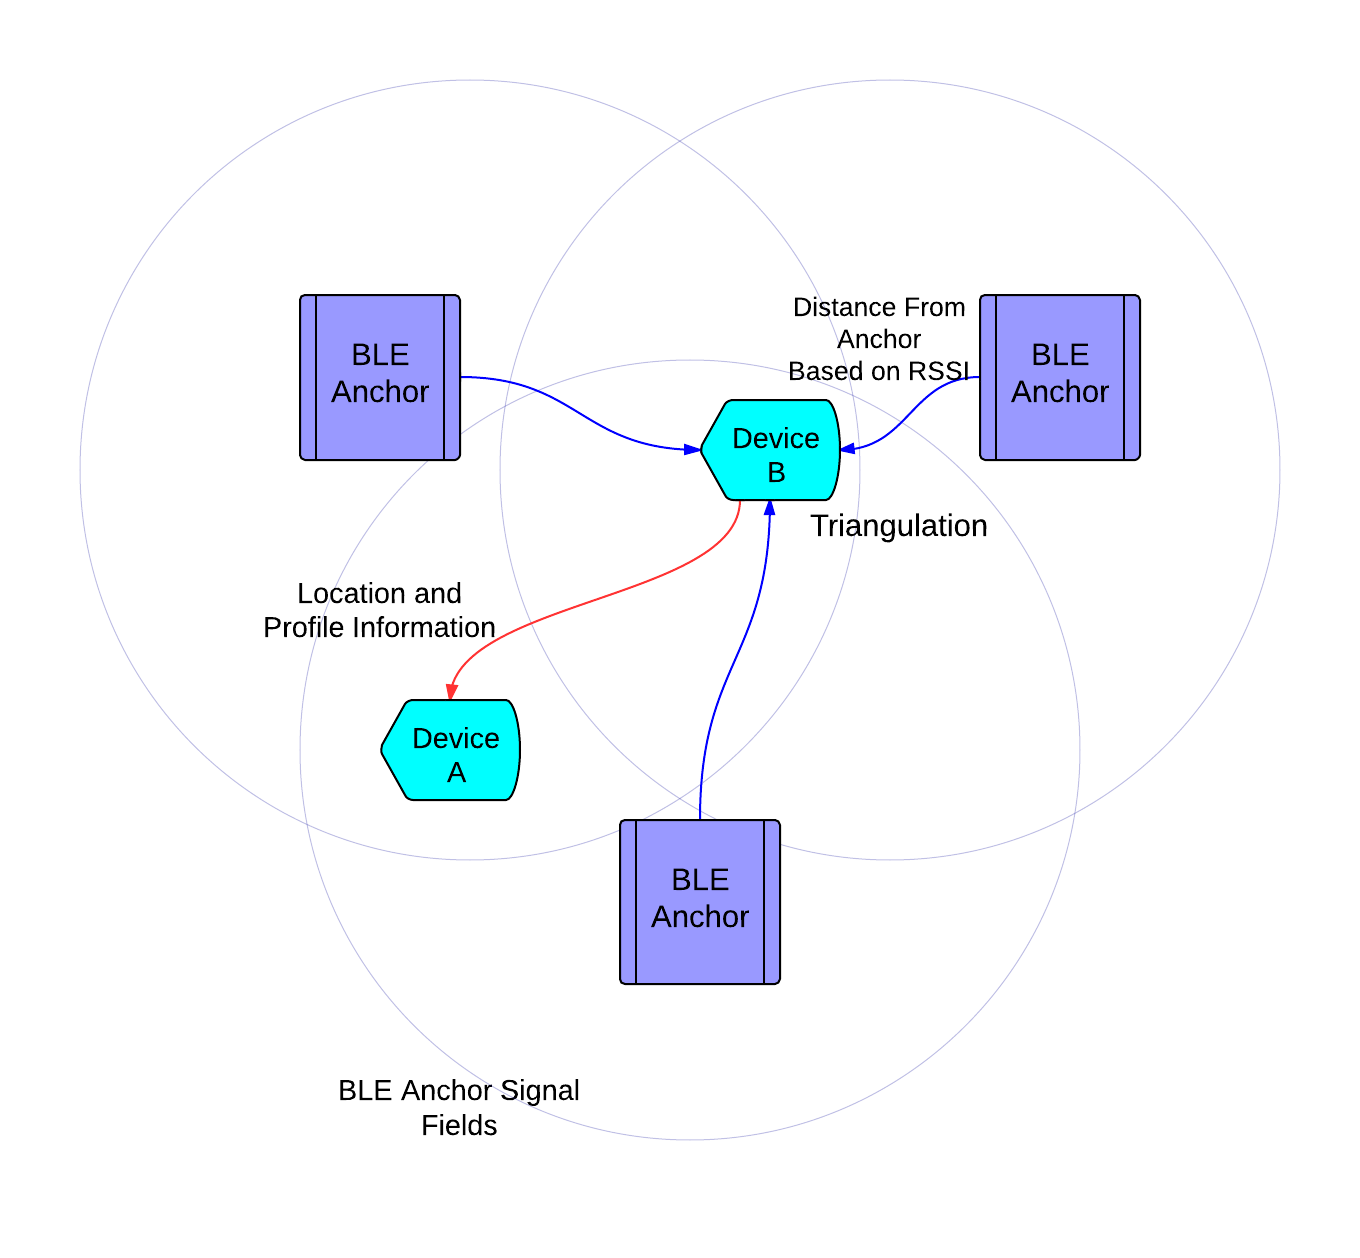
\includegraphics[width=1.00\linewidth]{blockflow}
	\end{center}
	\vspace{-12pt}
	\caption{Anticipated Approach to BLE Navigation}
	\label{fig:Block Flow Diagram}
\end{figure}

Three main modules must be put into place. First, the central
data processing unit will store all the relevant data pertaining to
the anchors. For example, in the shopping mall implementation, 
the product catalog and other information about 
the store would be associated with a partcular anchor, and then 
stored in the central data unit. The central data service will then
communicate with device, alerting it for example when an item
in the shopping list is nearby. It will also store the exact location
of each anchor, which it will use to calculate the position of a 
device when it comes into range of any anchor. The ideal 
structure that handles the central data service would be one that
can parse different pieces of data. 

Finally, the device to device communication must be well defined.
When a device enters the range of an anchor, the anchor should 
send over to the central data service information about itself (for
example, what products they currently have in stock) as well as the
location of the nearby device. Communication between devices
is also key; each device must be able to transmit profile information
to another device reliably.

The method we will use to caclulate location will be based of the 
Received Signal Strength Indicator (RSSI) that is associated with 
Bluetooth signal transmission. 

The use case we will base our project on is day to day use with 
friends. Those who have the app downloaded will be able to go 
into a room with a bluetooth device already set as an anchor, and 
be able to see which friends are in the room, and how to find them. 
The key features will be implemented through this use case, and 
the app can then be extended to handle more complex cases,
such as shopping mall navigation or emergency response. 
First, the anchor should be able to detect the device when it comes
into proximity; similarily, the device should recognize the anchor in
the room. Once recognized, the anchor will receive location data
(RSSI), and some contextual data from the detected device (for our
case we will use a user profile that includes name). The anchor 
will then send that data to our central data service, which will
then calculate the position of the device. Then, the central data
service will send back information about other devices and their
context. Essential here is that each bluetooth "message" holds
position data AND contextual data, and it will be transmitted from
device to device. 

\subsection{Technical Challenges}
\label{subsec:tech_challenges}
There are two main technical challenges involved with this project.
First, we have to build a functional app using fairly new technology, 
to implement an existing technique for navigaiton. Indoor navigation 
using BLE is unprecedented as mobile operating systems are just now 
providing APIs to use BLE as a geofencing tool. BLE itself was 
introduced in 2006, and it was only merged into the Bluetooth standard 
in 2010\footnote{bluetooth.com}. Even though BLE is in widespread use
today, the APIs to utilize BLE are very young

Calculating position using Bluetooth also poses an interesting problem.
"For a precise position estimation, the dependence between the distance 
and the received signal strength has to be determined. Especially in 
the indoor area, boundary conditions like reflections and wall damping
make the use of the equation for the free-field propagation impossible. 
Therefore, the required calculations of the distances are estimated by 
an approximation of the Received signal Strength Indicator (RSSI)"
\cite{feldman}. We must use a method to calculate position that has
been traditionally applied to older Bluetooth technology to the brand
new BLE 4.0. In addition, the new API may make this calculation
easier or harder; research and testing will be done on this.


\subsection{Evaluation Criteria}
\label{subsec:eval_criteria}
A fully functional BLE navigation app is certainly the most basic goal.
To demo this, we will be using two devices and an anchor to act as
our scenario. The anchor should detect the two devices and 
successfully send the contextual and RSSI data to the central
data service. Then, the data service should calculate the position
of all the devices and send back to each of the device its own location,
and the location of the other device, along with the user profile associated
with the other device.
In the end state, the two devices should know where they are, who 
the other device is, and where the other device is. Note additionally
that this should happen in real time; if device B moves, the user 
of the device A should see the movement.

As of the writing of this proposal, no BLE navigation applications are 
currently in widespread or mainstream use. During the course of
this project, that may change, and various BLE navigation applications 
may very well arise. We can compare results from these apps should
that happen. Also, since Android is currently the only operating system
who has opened to the public their BLE API, we will be using Android
devices to test all of this, and we will program the app for use on 
Android.


\section{Research Timeline}
\label{sec:research_timeline}
Since this project is much more focused on implementation over
research, most of the time will be devoted to building features of 
the end product. We will use agile processes (specifically, SCRUM 
with elements of extreme programming when meeting with our 
advisor) to complete our project.

The general format will follow two week sprint cycles, where a fully 
functional feature will be implemented by the end of each cycle. In
any given cycle, a feature will be implemented, tested, and refactored. 
Of course in the early stages, the emphasis will be on research
\begin{itemize*}
	\item {\sc already completed}: Preliminary reading. \vspace{3pt}
	\item {\sc prior-to thanksgiving} : Research on Bluetooth hardware, particularly how a solution will be implemented given the resources. Formulate the framework of the app - what platform will it be built on, what structures will be needed\vspace{3pt}
	\item {\sc prior-to christmas} : Have an API that fully implements BLE navigation - Detecting BLE transmitters is the main feature to accomplish.\vspace{3pt}
	\item {\sc completion tasks} : Verify implementation is bug-free. Conduct accuracy testing. Complete write-up.\vspace{3pt}
	\item {\sc if there's time} : Make the API relatively user/app friendly - ideally it needs to be
lightweight (we do not want BLE navigation consuming large amounts of resources), and easy to use
\end{itemize*}
Most of the research will involve the bluetooth hardware specifications, 
that is, the signal strength of BLE and the computational power of the 
everyday device.

\bibliographystyle{plain} 
\bibliography{prop_spec}  

\end{document} 

